\clearpage
\vspace*{\stretch{2}}%{\fill}
\begin{center}
\begin{minipage}{.75\textwidth}
\section{Análisis de la evaluación empírica}

Presentados la instalación del \emph{hardware} necesario y el análisis orgánico del software usado y programado desde cero, subrayar que por las características mínimas de la interfaz de usuario no es necesario dedicar más análisis que el realizado hasta el momento. En este capítulo presentamos los resultados experimentales de la evaluación del sistema con distintos tipos de terminales móviles. % \pagebreak
\end{minipage}
\end{center}
\vspace{\stretch{3}} % \vfill % equivalent to \vspace{\fill}
\clearpage% https://tex.stackexchange.com/questions/70714/center-horizontally-and-vertically-a-block-of-text

\subsection{Resultados con una tableta Android}
A continuación se muestra cómo un dispositivo portátil (en este caso una \emph{tablet} Samsung Galaxy GP-P5210, de 1 GB de RAM y con el sistema operativo Android 4.4.2) puede enviar su audio, recibir las credenciales en respuesta y conectarse a Internet. Las pruebas se hicieron con el navegador Chrome 61 y se monitorizaron los procesos con las herramientas de depuración remota de \emph{Chrome DevTools} \cite{ChromeDevTools}.
 
En la Figura \ref{connectionChilli} se muestran resaltados los datos relevantes en el proceso de conexión exitoso, en orden descendiente, correspondientes al guardado y envío de audio, recepción de credenciales y conexión con éxito, como revela el código de estado 1 al llamar a la función \emph{logon()}.

\begin{figure}[!t]
\begin{center}
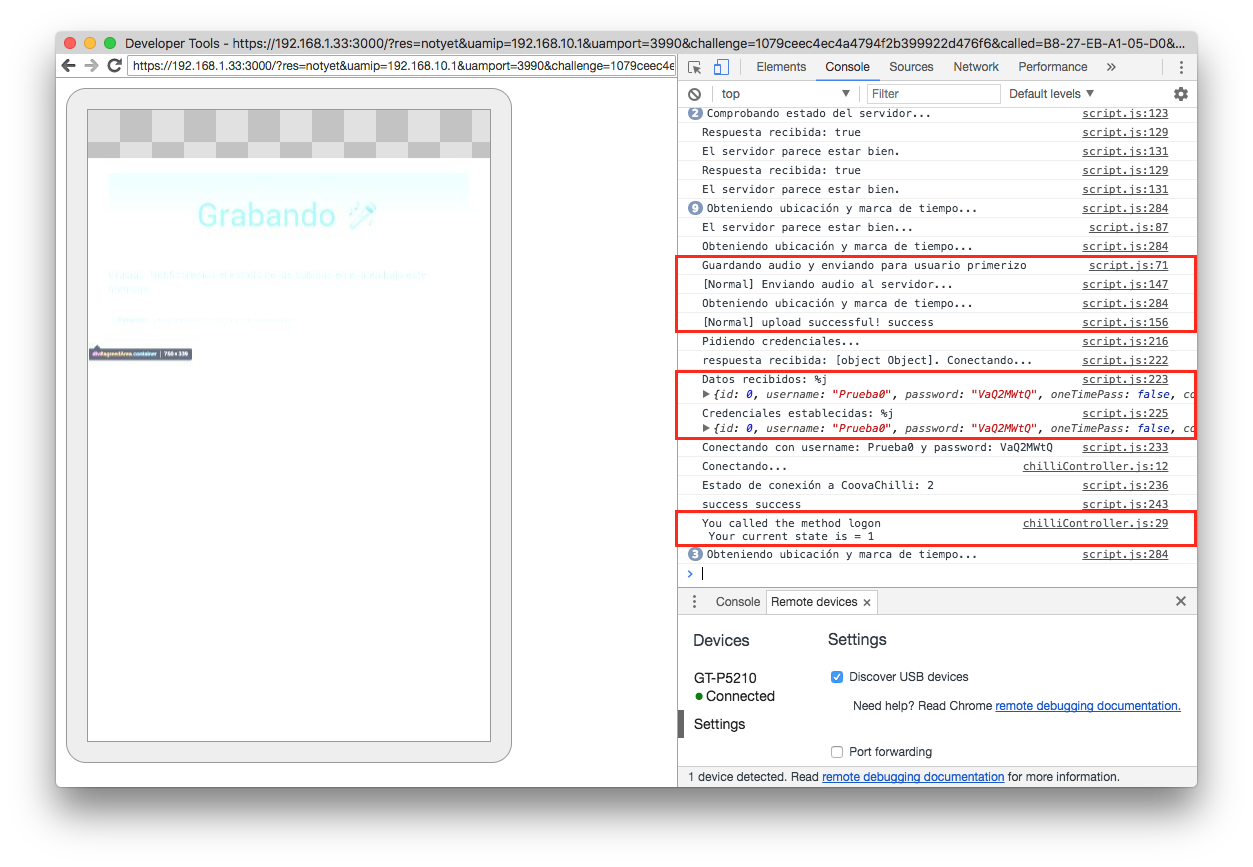
\includegraphics[width=0.75\linewidth]{./6_EvalEmpirica/Img/connectionChilli.png}
\end{center}
\caption{Datos relevantes del proceso de conexión con éxito de una tableta Android}
\label{connectionChilli}
\end{figure}

Como se puede apreciar, cuando se envía el fichero de audio generado al servidor este responde con un objeto JavaScript que contiene las credenciales del tipo de usuario seleccionado. Tras recibir estos datos, el sistema realiza el \emph{login} con dichas credenciales, conectando al usuario a internet (como puede verse en el código de estado de la conexión, que es 1).

Dado que el proceso de desconexión automática implica cerrar la pestaña, lo que cancelaría la sesión de depuración en curso, se realizó una desconexión manual llamando a la función \emph{logoff()}. En la captura puede verse por orden descendiente el estado actual de la conexión a Internet tras llamar a la función \emph{refresh()} y la llamada a la función de desconexión y el código de estado resultante a estar desconectado (Figura \ref{chilliDisconnect}).

\begin{figure}[!t]
\begin{center}
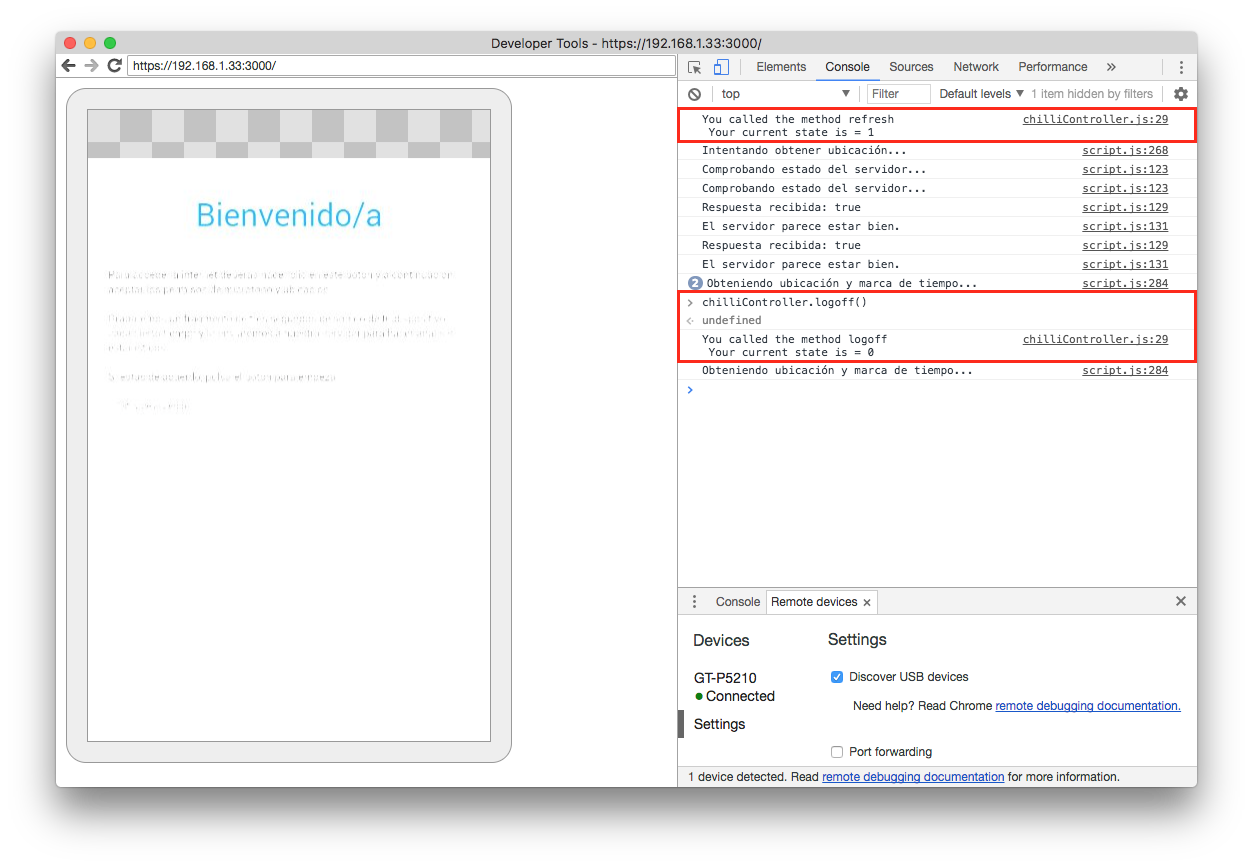
\includegraphics[width=0.75\linewidth]{./6_EvalEmpirica/Img/chilliDisconnect.png}
\end{center}
\caption{Proceso de desconexión}
\label{chilliDisconnect}
\end{figure}

\subsection{Consumo de RAM del sistema en la Raspberry Pi}

Tras realizar las pruebas de funcionamiento pertinentes se analizó el consumo total de memoria de los procesos implicados en la implantación del sistema. Utilizando la herramienta \emph{htop}, disponible en sistemas Linux y que monitoriza la memoria física, memoria virtual, memoria de intercambio \emph{swap} y consumo de CPU tanto en valor absoluto como en porcentajes entre otras muchas cosas, se monitorizaron las estadísticas concernientes a las instancias de Node.js, \emph{hostapd}, \emph{CoovaChilli} y la estructura en la que se apoya: \emph{freeRADIUS} y \emph{MySQL}.

En la Figura \ref{htopGeneric} se muestra la ventana genérica al ejecutar el comando \emph{htop} desde el terminal.

\begin{figure}[!t]
\begin{center}
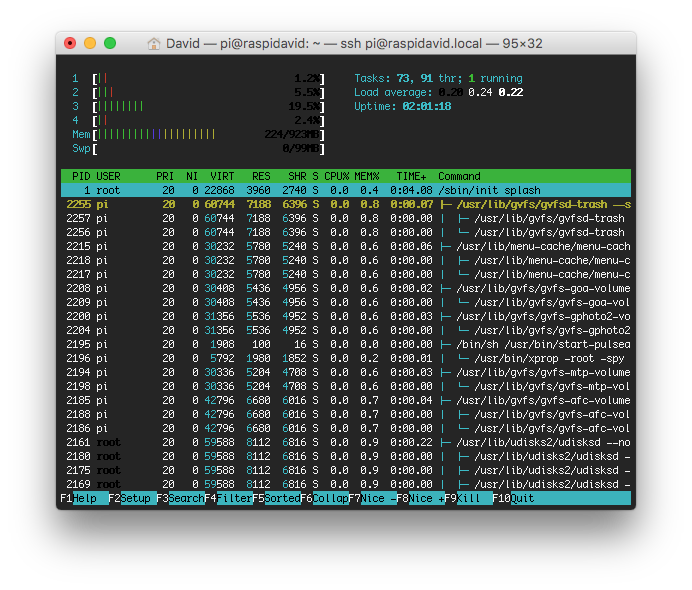
\includegraphics[width=0.75\linewidth]{./6_EvalEmpirica/Img/htopGeneric.png}
\end{center}
\caption{Ventana genérica para la orden htop}
\label{htopGeneric}
\end{figure}

En la Figura \ref{htopNode} se muestra el consumo de recursos de Node.js.

\begin{figure}[!t]
\begin{center}
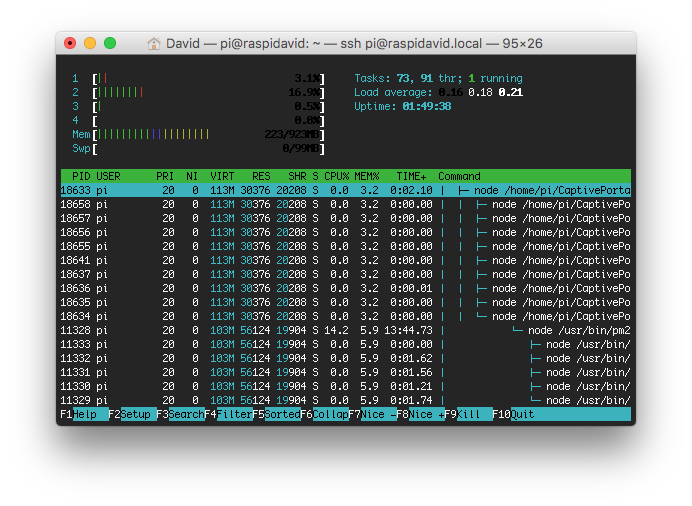
\includegraphics[width=0.75\linewidth]{./6_EvalEmpirica/Img/htopNode.png}
\end{center}
\caption{Consumo de recursos de Node.js}
\label{htopNode}
\end{figure}

En esta captura puede apreciarse cómo el proceso que controla la instancia de la utilidad PM2 (que a su vez es la que controla la ejecución de nuestra instancia de \emph{node}) es la que destaca en el uso de recursos, utilizando un porcentaje de memoria del 5.9\% y un 14.2\% de la CPU. Lo que supone un bajo consumo.

En la Figura \ref{pm2monitNode} se muestra una cifra más inmediata del consumo total de nuestro proceso con la propia utilidad PM2, resaltada en azul en el campo superior izquierdo del monitor llamado con el comando \emph{pm2 monit} (que se explica en el Anexo C). Que también se observa que es muy reducido.

\begin{figure}[!t]
\begin{center}
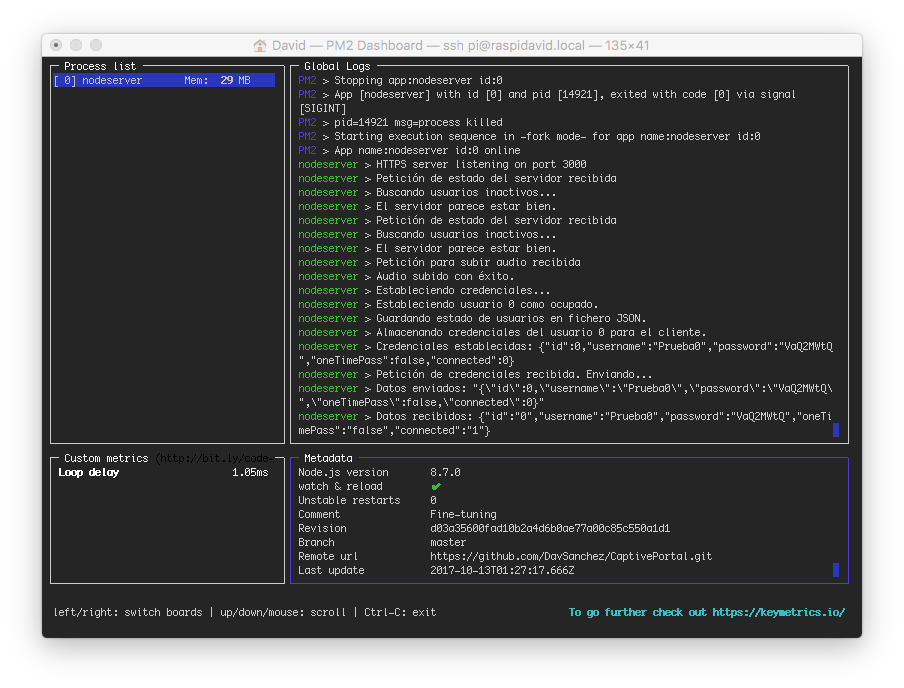
\includegraphics[width=0.75\linewidth]{./6_EvalEmpirica/Img/pm2monitNode.png}
\end{center}
\caption{Ventana de consumo usando la orden pms monit}
\label{pm2monitNode}
\end{figure}

En la Figura \ref{htopChilli} se muestra el consumo de recursos de CoovaChilli. Se puede observar que el proceso correspondiente a CoovaChilli es ligero, no ocupando apenas procesador y un porcentaje muy bajo de la memoria total de la Raspberry Pi.

\begin{figure}[!t]
\begin{center}
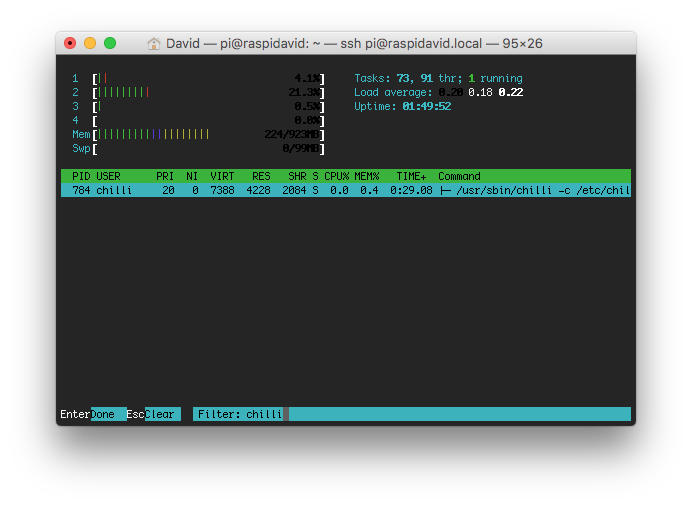
\includegraphics[width=0.75\linewidth]{./6_EvalEmpirica/Img/htopChilli.png}
\end{center}
\caption{Consumo de procesador y memoria de CoovaChilli}
\label{htopChilli}
\end{figure}

En la Figura \ref{htopRADIUS} se muestra el consumo de recursos de freeRADIUS. Se puede observar que consume poco procesador, aunque su consumo en memoria es varias veces mayor al de CoovaChilli.

\begin{figure}[!t]
\begin{center}
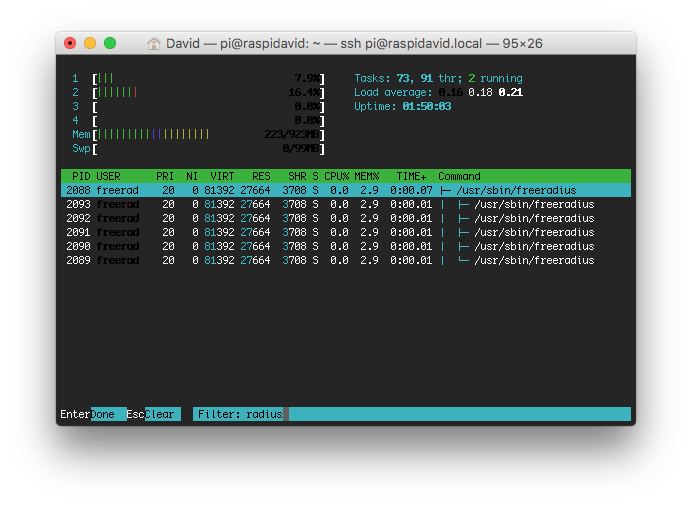
\includegraphics[width=0.75\linewidth]{./6_EvalEmpirica/Img/htopRADIUS.png}
\end{center}
\caption{Consumo de procesador y memoria de freeRADIUS}
\label{htopRADIUS}
\end{figure}

En la Figura \ref{htopMySQL} se muestra el consumo de recursos de MySQL. Tal y como sucede con freeRADIUS, el consumo de procesador es muy bajo aunque su consumo de memoria es de hasta diez veces mayor al de CoovaChilli. Lo cual es lógico porque CoovaChilli requiere únicamente el almacenamiento de muy pocos datos relativos a conversiones de direcciones IP, en cambio ya únicamente el motor de la MySQL requiere de mucha más memoria.

\begin{figure}[!t]
\begin{center}
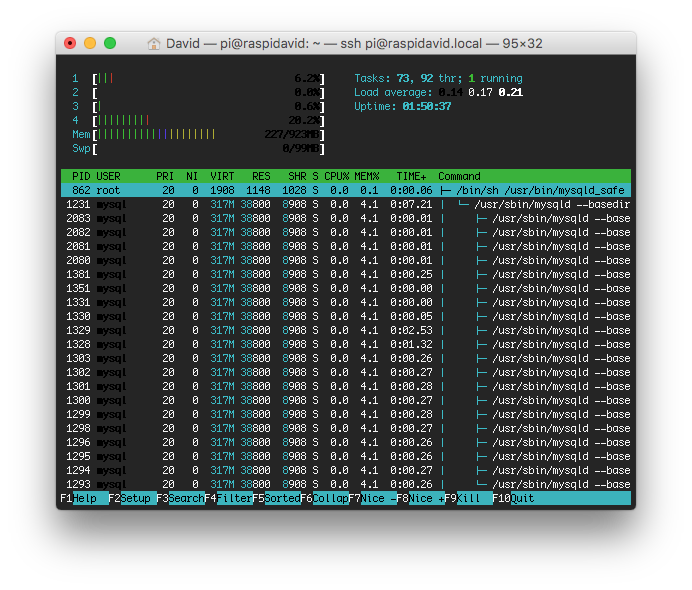
\includegraphics[width=0.75\linewidth]{./6_EvalEmpirica/Img/htopMySQL.png}
\end{center}
\caption{Consumo de procesador y memoria de MySQL}
\label{htopMySQL}
\end{figure}

Por último, en la Figura \ref{htopHostapd} mostramos los recursos utilizados por \emph{hostapd}, cuyas estadísticas de consumo son similares al proceso de CoovaChilli.

\begin{figure}[!t]
\begin{center}
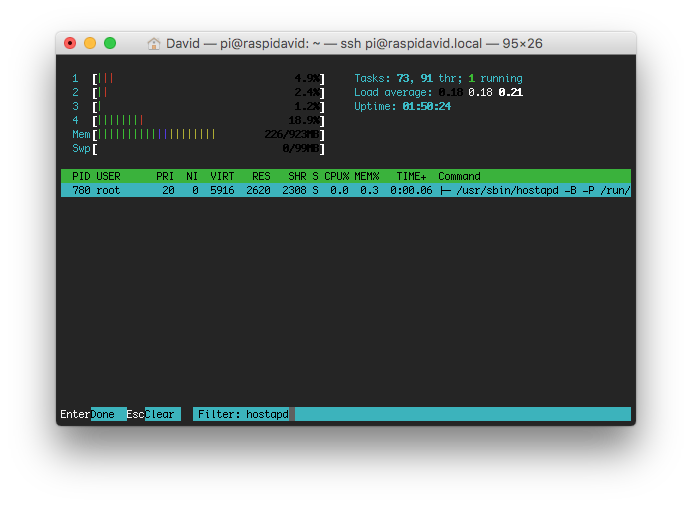
\includegraphics[width=0.75\linewidth]{./6_EvalEmpirica/Img/htopHostapd.png}
\end{center}
\caption{Consumo de procesador y memoria de Hostapd}
\label{htopHostapd}
\end{figure}

Con estos datos podemos considerar que el sistema implementado consume aproximadamente el 15\% de los recursos del procesador y memoria RAM de la Raspberry Pi 3. Sin embargo, hay que tener en cuenta que, aparte de un ligero sobredimensionamiento de los porcentajes, muchos procesos no se dedican exclusivamente al mantenimiento de nuestro sistema, pudiendo estar consumiendo las cantidades de recursos mostradas aquí debido a que también se dedican a otras funciones (como puede ser el caso de las múltiples instancias de los procesos de MySQL).


\subsection{Consumo de RAM de los navegadores Web}

Aparte del consumo de recursos del servidor, también se estudió el consumo de recursos del sistema con el que los clientes se conectan a nuestro servicio, que en este caso no es otra cosa que el navegador Web.

En la Figura \ref{tabletChrome} se muestra una captura de ventana de uno de los dispositivos móviles utilizados, una tablet Samsung Galaxy GP-P5210, de 1 GB de RAM, con Android 4.4.2 y el navegador Chrome 61.

\begin{figure}[!t]
\begin{center}
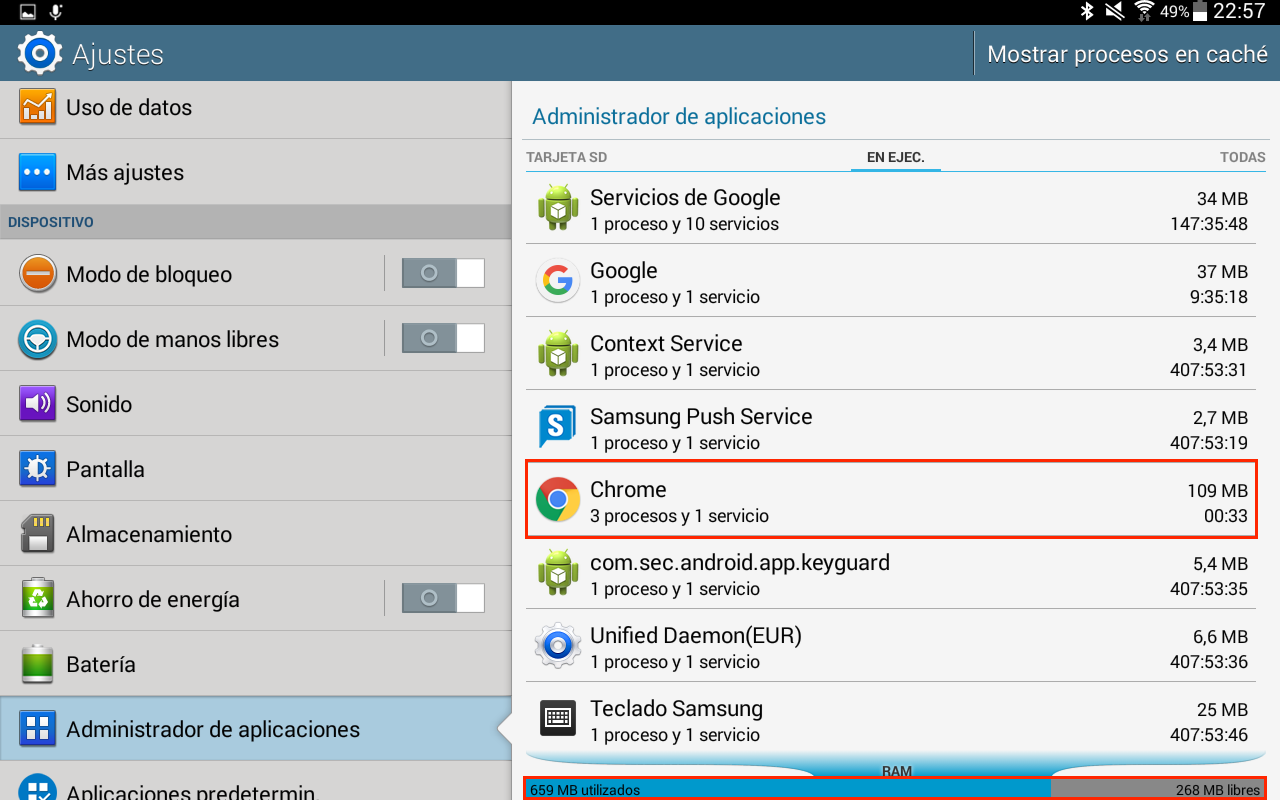
\includegraphics[width=0.75\linewidth]{./6_EvalEmpirica/Img/tabletChrome.png}
\end{center}
\caption{Ventana de consumo de RAM de los navegadores Web en una tablet Android}
\label{tabletChrome}
\end{figure}

En las pruebas de escritorio se ha analizado el consumo de los navegadores Mozilla Firefox 57 y Vivaldi 1.12 en un equipo con macOS 10.12.6, de 16 GB de RAM, y Microsoft Edge en un equipo con Windows 10 con 8 GB. En la Figura \ref{firefoxRAM} se muestra el consumo de RAM en Mozilla Firefox para MacOS, resaltado en azul. El consumo de RAM de esta versión de Firefox puede parecer elevado sobre todo si lo comparamos con el consumo en la tablet, ya que incluso el consumo sin ningún contenido abierto y en una red diferente es tan solo entre 25 y 75 MB menor. Esto se debe en parte a las extensiones específicas y herramientas de desarrollador que vienen instaladas por defecto en esta versión.

\begin{figure}[!t]
\begin{center}
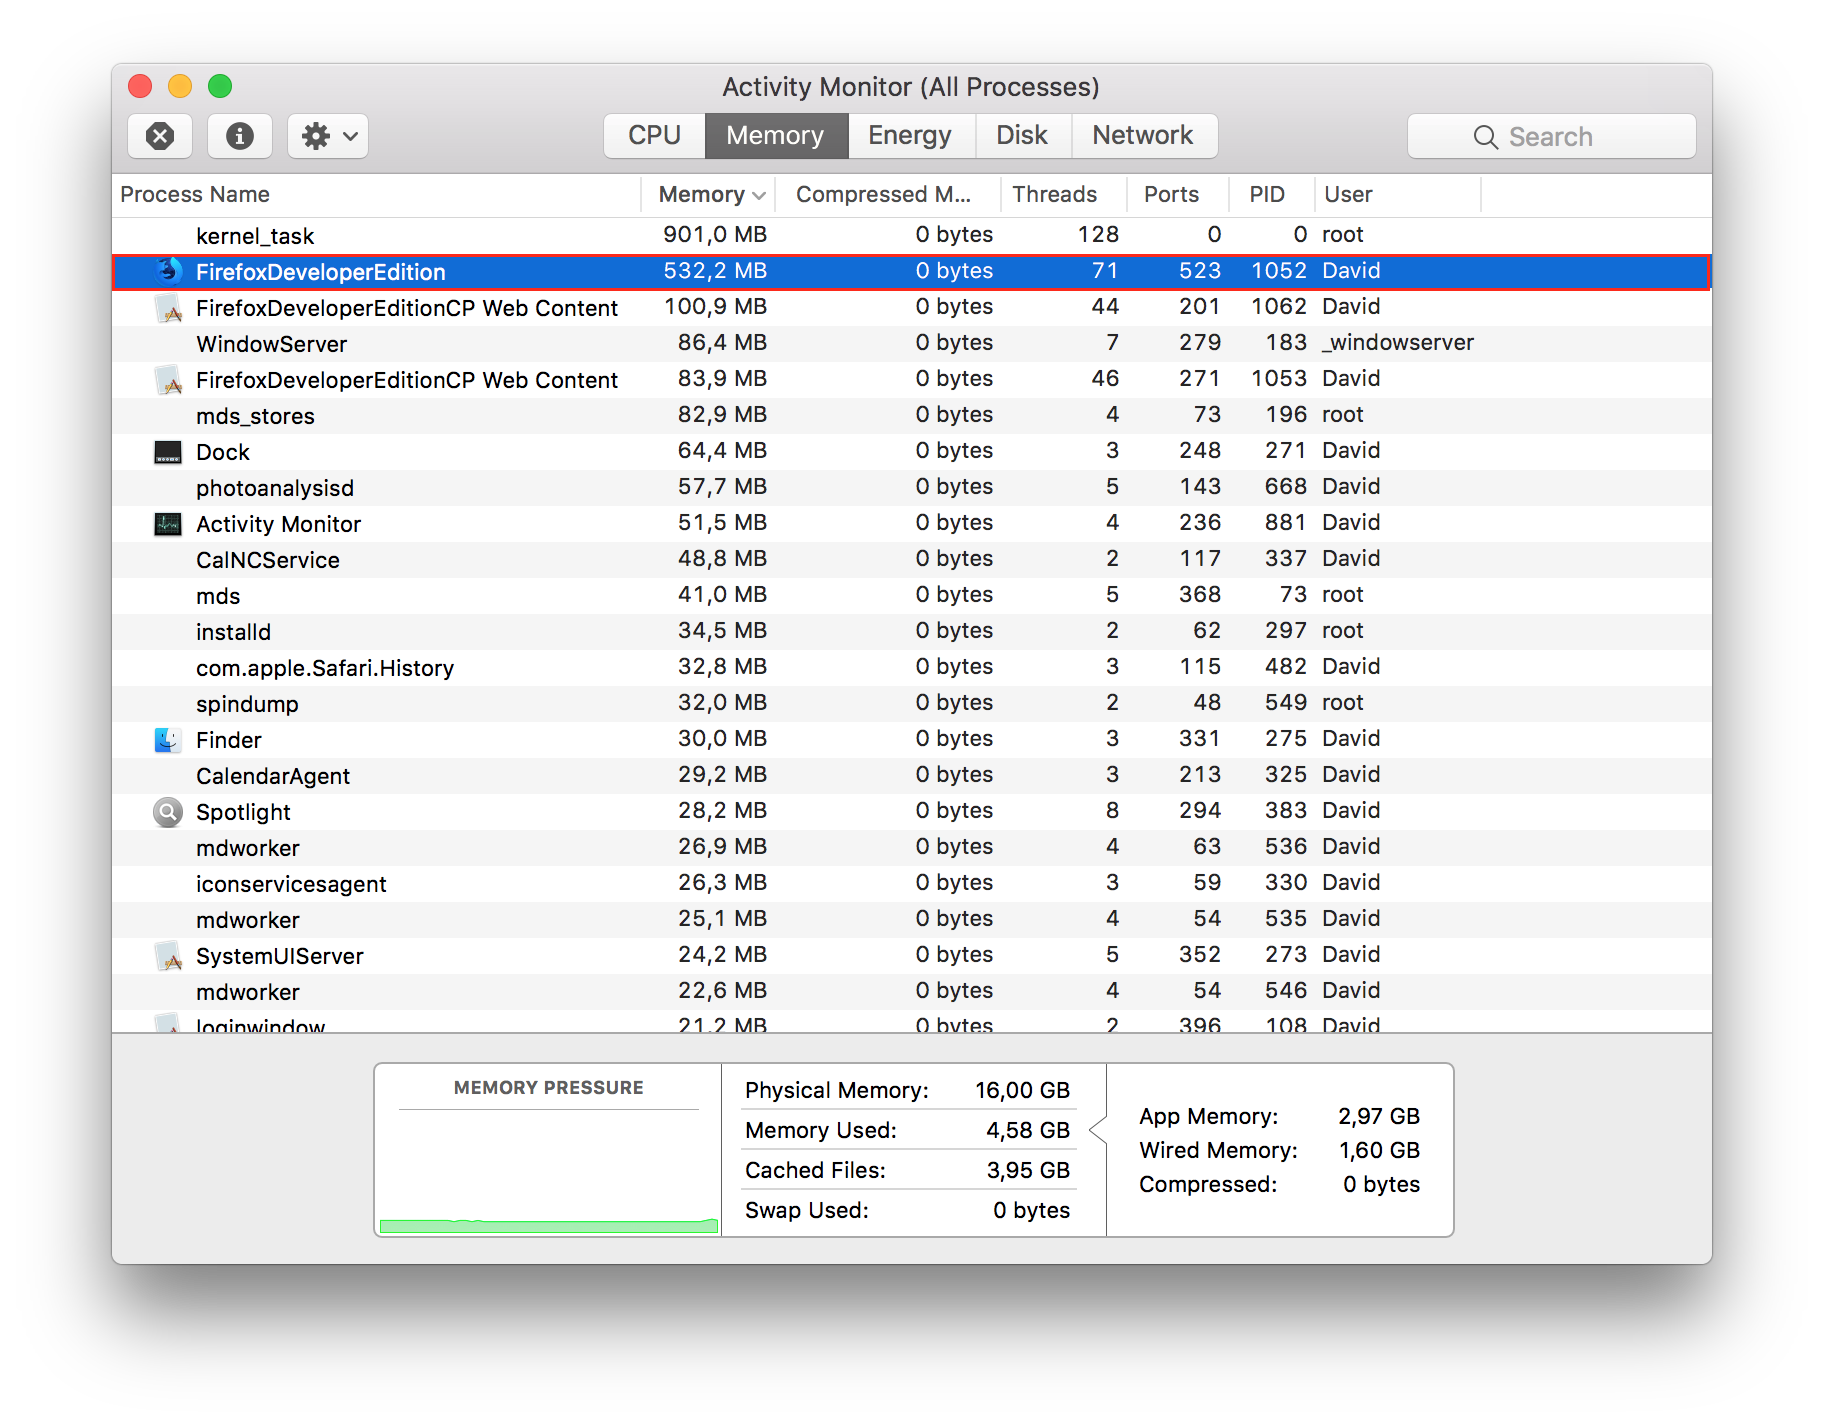
\includegraphics[width=0.75\linewidth]{./6_EvalEmpirica/Img/firefoxRAM.png}
\end{center}
\caption{Consumo de RAM de Mozilla Firefox para un computador MacOS}
\label{firefoxRAM}
\end{figure}

El consumo de recursos en Vivaldi sin extensiones ni complementos se mantiene en unas cifras inferiores sin tener en cuenta la presencia de los Vivaldi Helpers, aunque en total el consumo sigue siendo inferior a Firefox en escritorio y superior a Chrome en Android (Figura \ref{vivaldiRAM}).

\begin{figure}[!t]
\begin{center}
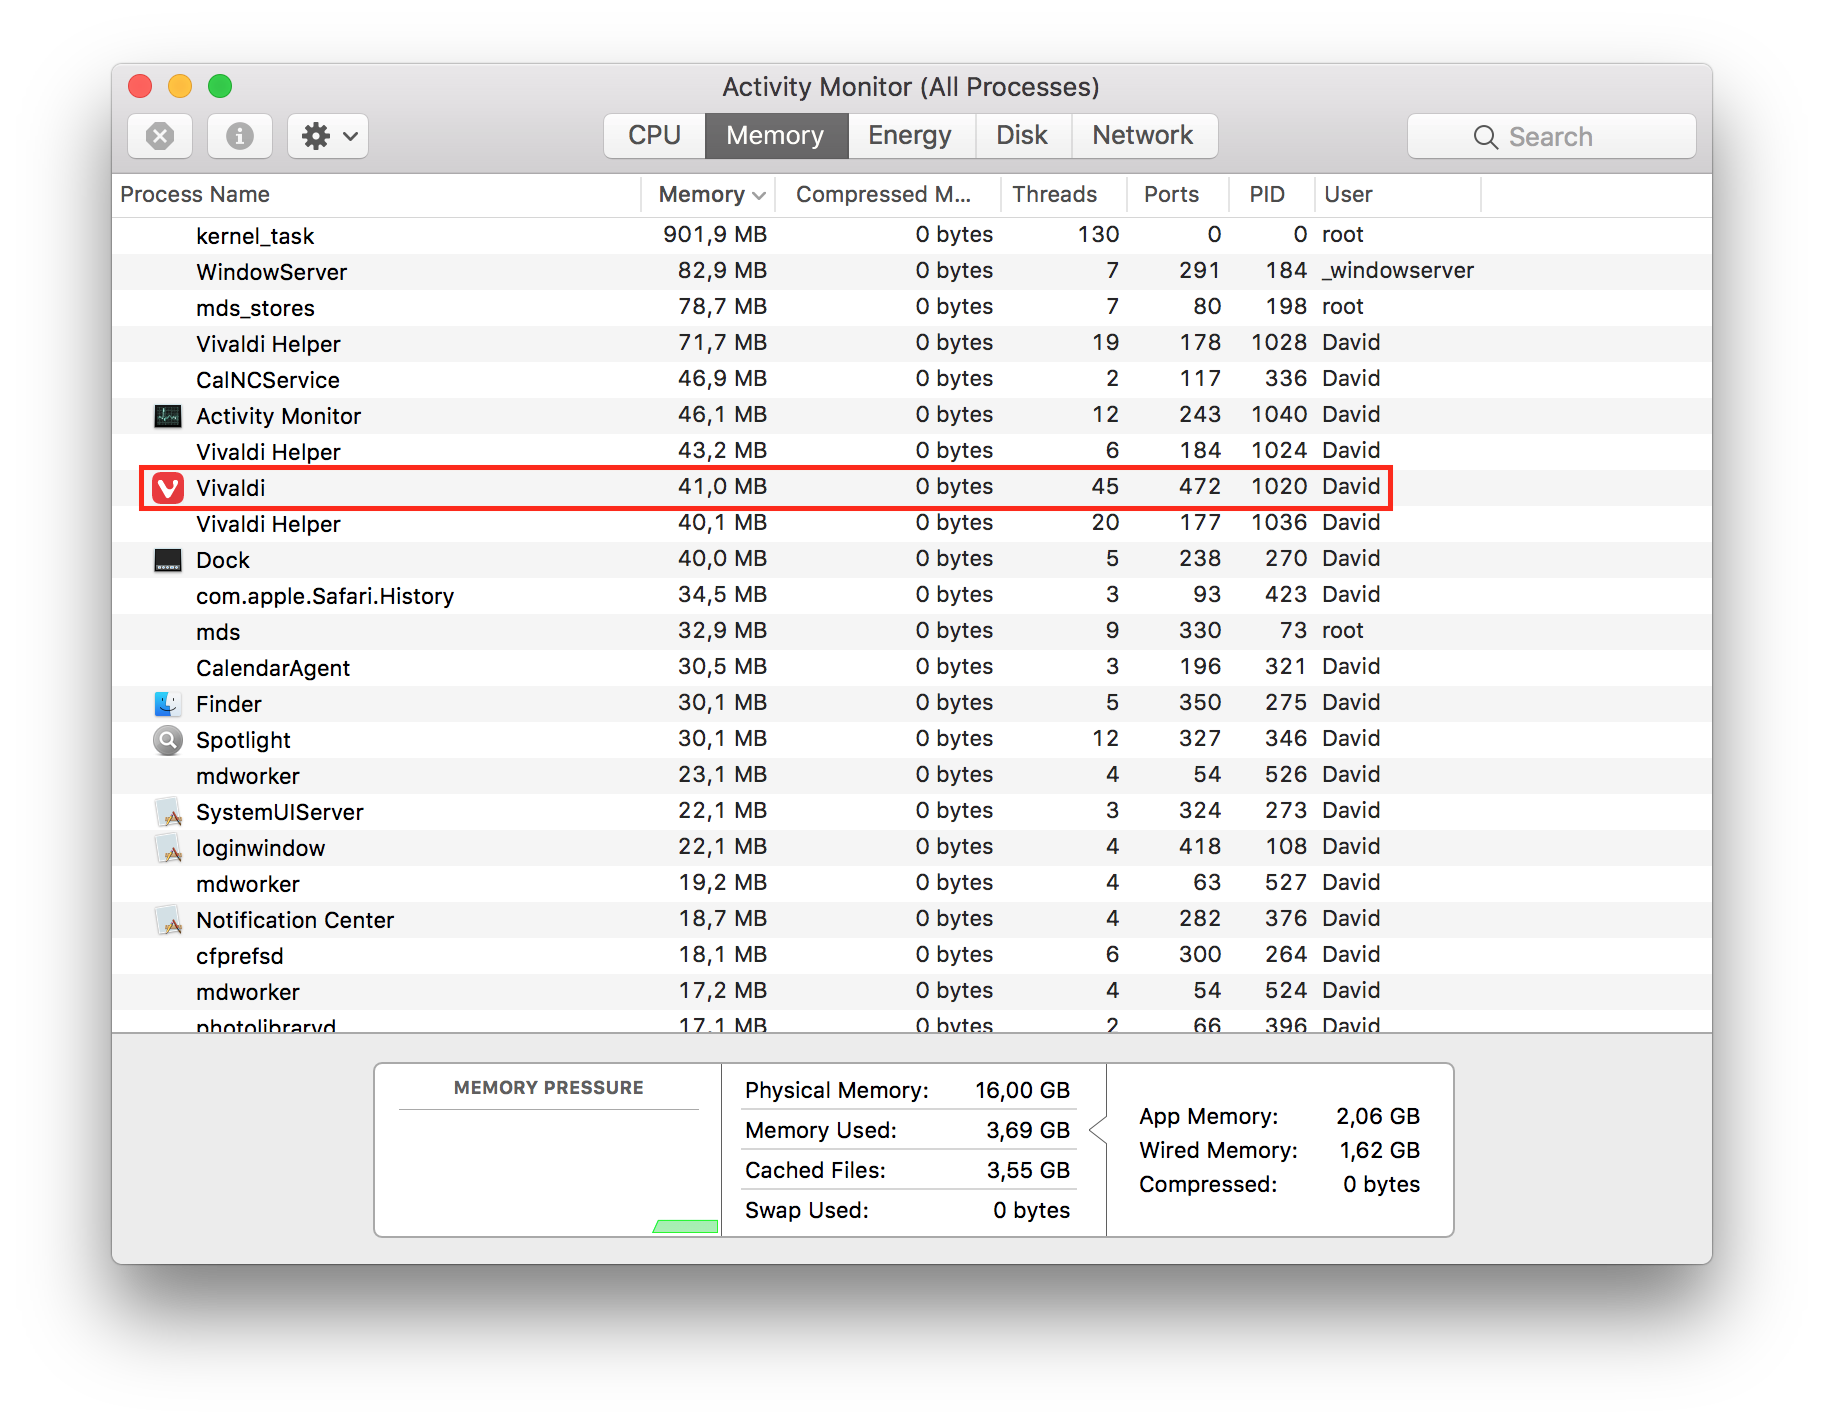
\includegraphics[width=0.75\linewidth]{./6_EvalEmpirica/Img/vivaldiRAM.png}
\end{center}
\caption{Consumo de RAM de Vivaldi para un computador MacOS}
\label{vivaldiRAM}
\end{figure}

El consumo de RAM en Microsoft Edge, resaltado en rojo, es mucho menor. Dado que la transferencia de archivos de audio por la red ocurre de forma puntual y a intervalos muy cortos de tiempo, los indicadores de consumo de red son nulos en el momento de tomar la captura debido a que se encontraban entre envíos (Figura \ref{edgeRAM}).

\begin{figure}[!t]
\begin{center}
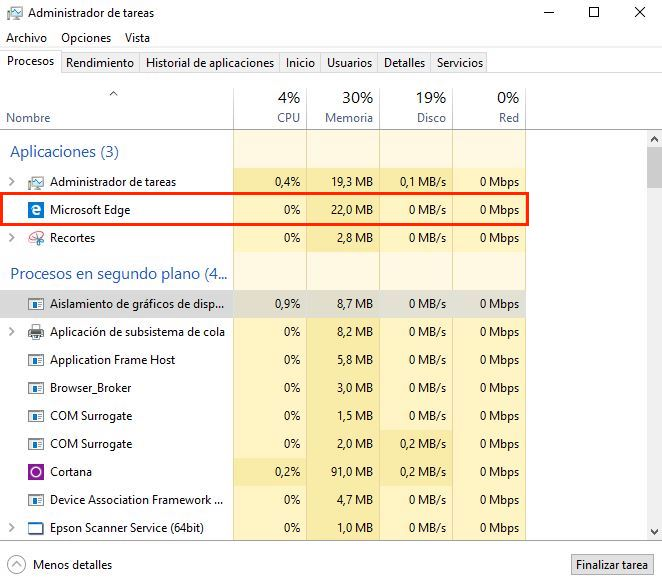
\includegraphics[width=0.75\linewidth]{./6_EvalEmpirica/Img/edgeRAM.jpg}
\end{center}
\caption{Consumo de RAM de Microsoft Edge para un computador con Windows}
\label{edgeRAM}
\end{figure}

\subsection{Tráfico HTTP y TCP}

En una de las pruebas del sistema con el navegador de escritorio Firefox y cuando aún no se había implementado SSL se realizó una captura del tráfico con Wireshark. En la Figura \ref{traffic} se muestra el \emph{throughput} medio de la transmisión de audio desde el navegador al servidor, consistente en 45 tramas TCP de una longitud total de 64206 bits.

\begin{figure}[!t]
\begin{center}
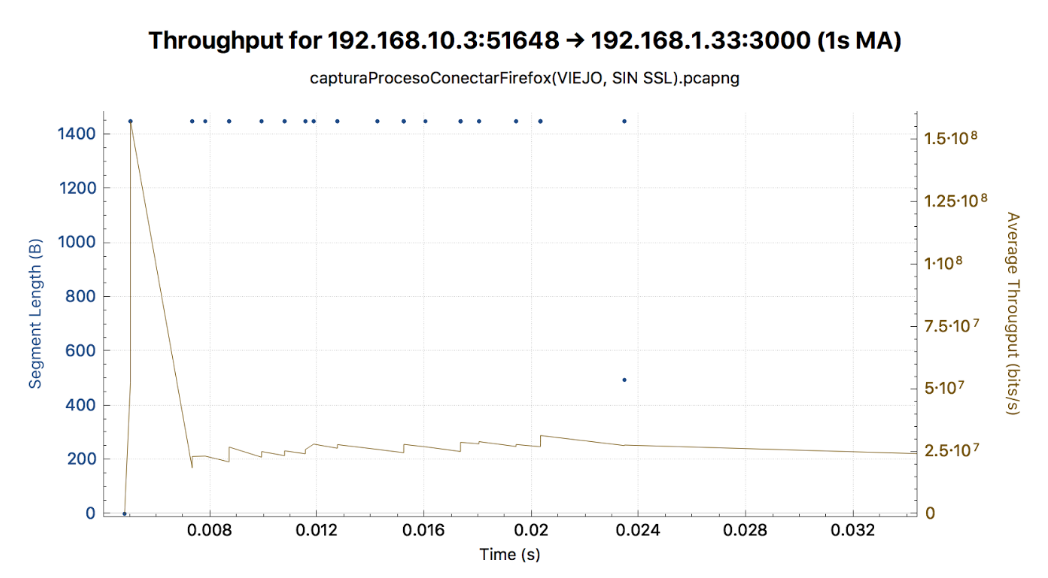
\includegraphics[width=0.75\linewidth]{./6_EvalEmpirica/Img/traffic.png}
\end{center}
\caption{Throughput de tráfico TCP y HTTP para comunicación de un archivo de audio}
\label{traffic}
\end{figure}

Además, en las pruebas con sistemas de escritorio se realizó una prueba de velocidad del cliente conectado a través de nuestro sistema y se comparó con pruebas de velocidad cuando el usuario está conectado al mismo servicio contratado a la WiFi tradicional proporcionada por el equipo del operador. Las cifras para la conexión inalámbrica cuando se usa nuestro sistema en la comparativa descienden en 10 Mbps tanto en subida como en bajada, lo que es esperable dado que estamos añadiendo varias capas más de procesamiento a la transmisión (Figura \ref{speed}).

\begin{figure}[!t]
\begin{center}
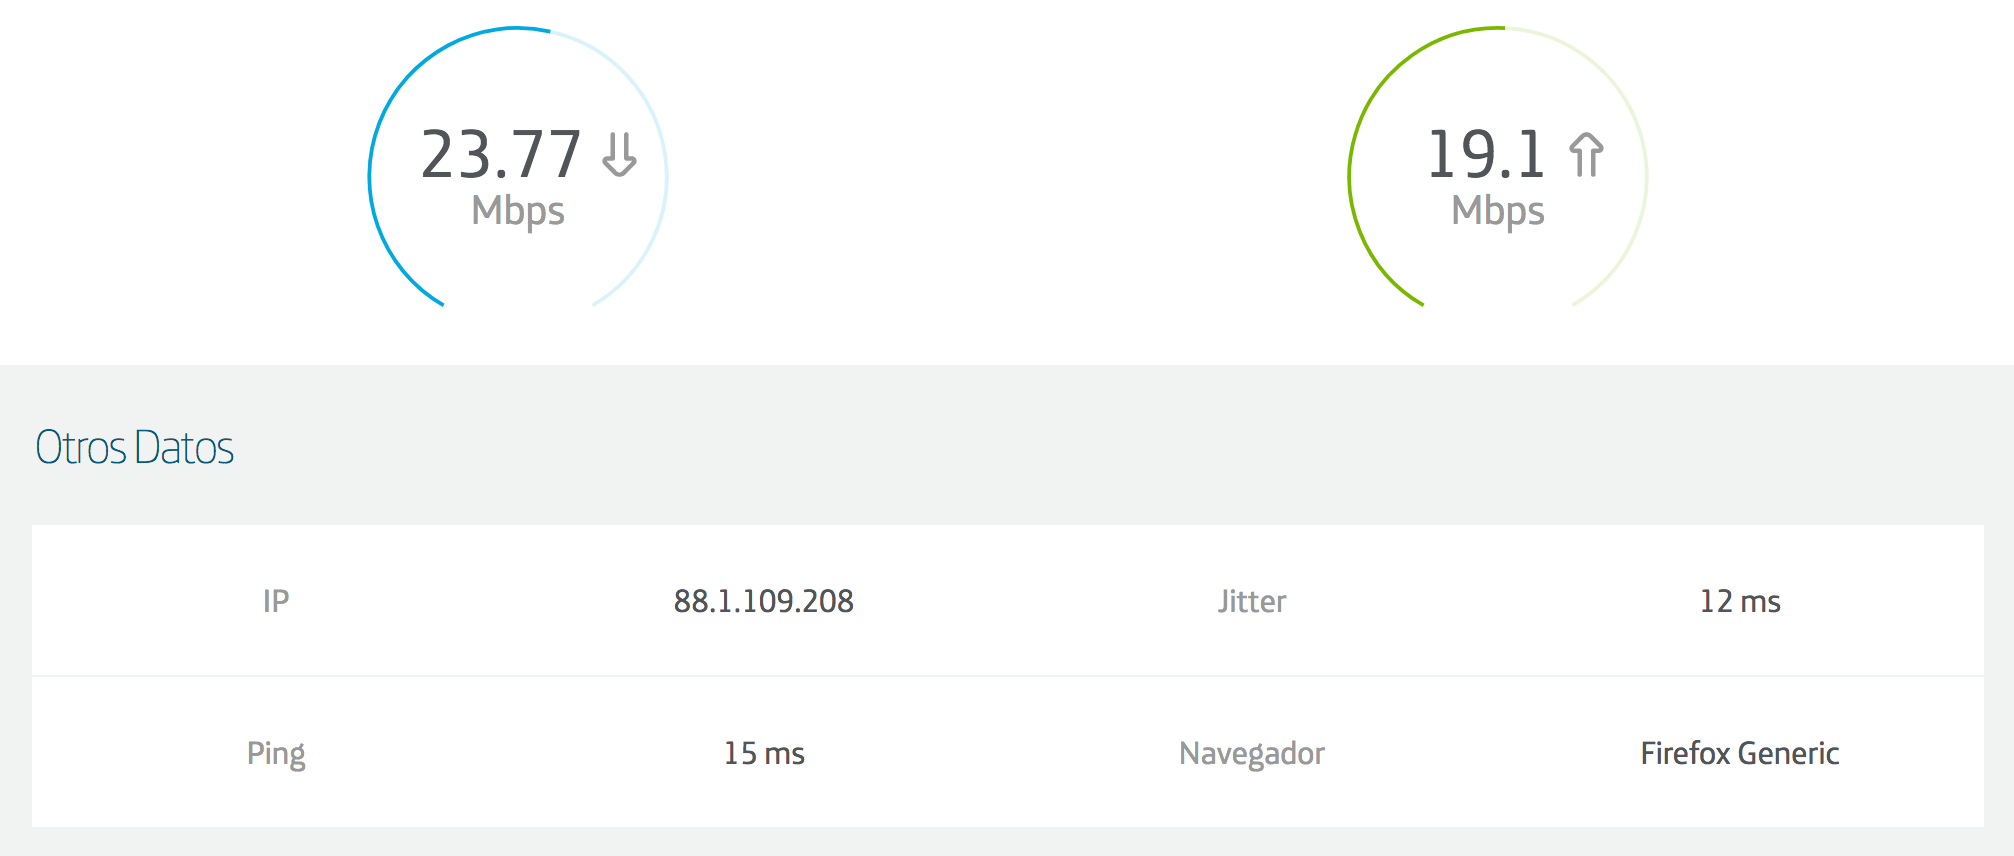
\includegraphics[width=0.75\linewidth]{./6_EvalEmpirica/Img/speed.png}
\end{center}
\caption{Prueba de velocidad de acceso a Internet a través de nuestro sistema}
\label{speed}
\end{figure}

\subsection{Análisis de los archivos de audio generados}
Los archivos de audio generados y enviados al servidor son renombrados por la \emph{Aplicación Web} siguiendo la estructura de la Figura \ref{audioFiles}: el prefijo \emph{Lat} seguido de la latitud, el prefijo \emph{Lon} seguido de la longitud y el prefijo \emph{Time} seguido del \emph{timestamp} completo.

\begin{figure}[!t]
\begin{center}
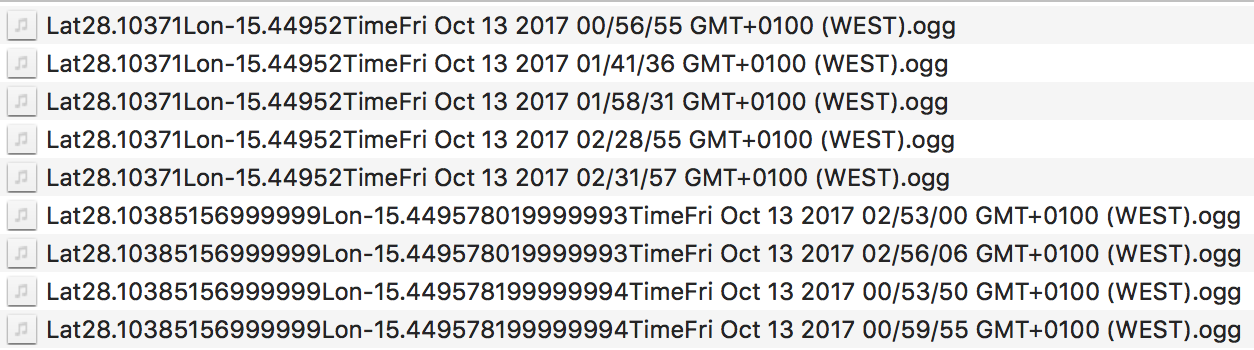
\includegraphics[width=0.75\linewidth]{./6_EvalEmpirica/Img/audioFiles.png}
\end{center}
\caption{Formato del archivo de audio etiquetado con geolocalización y temporización}
\label{audioFiles}
\end{figure}

Cada archivo tiene una duración de 4 segundos, está codificado en \emph{Opus Audio} \cite{OpusCodec} y almacenado en un contenedor de formato \emph{Ogg}. La tasa de muestreo de la codificación es \emph{fullband} (48 kHz, como puede verse en la imagen). El fichero generado ronda los 63 KB de tamaño, lo que confirma lo apreciado en la captura del tráfico TCP correspondiente a un fichero enviado, de tamaño total ligeramente mayor y dividido en varias tramas (Figura \ref{audioInfo}).

\begin{figure}[!t]
\begin{center}
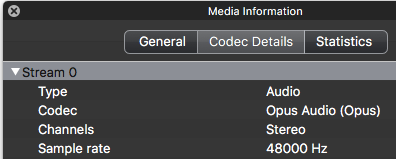
\includegraphics[width=0.75\linewidth]{./6_EvalEmpirica/Img/audioInfo.png}
\end{center}
\caption{Codificación del audio}
\label{audioInfo}
\end{figure}